\documentclass{article} % For LaTeX2e
\usepackage{nips15submit_e,times}
\usepackage{hyperref}
\usepackage{url}
\usepackage{graphicx}
\usepackage{amsmath}
\graphicspath{ {./} }
%\documentstyle[nips14submit_09,times,art10]{article} % For LaTeX 2.09


\title{Attention Pooling and Latent Space Analysis of WSI BYOL Embeddings}


\author{
John Miller \\
Mt. Sinai School of Medicine\\
\texttt{john.miller@icahn.mssm.edu} \\
\And
Gabe Marx \\
Mt. Sinai School of Medicine \\
\texttt{gabriel.marx@icahn.mssm.edu} \\
}

% The \author macro works with any number of authors. There are two commands
% used to separate the names and addresses of multiple authors: \And and \AND.
%
% Using \And between authors leaves it to \LaTeX{} to determine where to break
% the lines. Using \AND forces a linebreak at that point. So, if \LaTeX{}
% puts 3 of 4 authors names on the first line, and the last on the second
% line, try using \AND instead of \And before the third author name.

\newcommand{\fix}{\marginpar{FIX}}
\newcommand{\new}{\marginpar{NEW}}

%\nipsfinalcopy % Uncomment for camera-ready version

\begin{document}


\maketitle

\begin{abstract}
By combining recent developments in the field of computer vision, we generated a paradigm which utilizes slide-level-labels to categorize tau burden in whole slide images. Given the enormity of these WSIs (up to 40,000 by 40,000 pixels), computational modeling is largely impossible on the whole image outside of top of the line hardware. We previously created a self-supervised feature learning paradigm which could extract features from tiles drawn from WSIs, and present the WSI as a composite of its tiles. We refine our approach here by introducing an attention pooling method to the classification of these combined embeddings, improving performance markedly and achieving an RMSE of \textbf{0.61} on a slide-level ordinal regression task. Additionally, we perform latent space analysis of our self-supervised embeddings and reveal that they are much more feature-rich than originally anticipated, eallowing for the extraction of anatomical information on top of the original tau burden scope.
\end{abstract}

\section{Introduction}

Pathology is one of the last medical fields to join the digital revolution of medicine. The recent digitization of whole slide images (WSI) has opened opportunities for computational approaches to pathology problems. However, due to the recency of digital pathology there is a severe lack of annotated datasets. Acquisition of detailed pathology annotations presents a unique challenge. Each WSI, often scanned at 20x magnification (0.5 microns per pixel), contains several gigapixels of data. Detailed annotations of a single WSI could take several hours for a trained pathologist to perform. Additionally, their size provides a significant obstacle to computational modeling, as single images can take up prohibitively large amounts of memory. One approach to this problem is using a weakly supervised approach to training in which a single label is used for an entire WSI’s worth of data. In this paradigm, a WSI is broken down into small (256x256 pixel) tiles. At prediction time, tiles are pooled into a single instance which represents the WSI along with its representative label. 

While the field of oncopathology has fully harnessed weakly and self supervised learning, it has yet to be applied to neuropathology. Specifically, in the subfield of neurodegenerative neuropathology, brain banks across the country collect hundreds of thousands of WSIs. Considering that about 470 WSIs contain roughly the same number of pixels as the entire ImageNet dataset, this represents an incredible amount of data which, if properly harnessed, can be used to answer many of the unsolved questions about the neurodegenerative disease process, bringing the field closer to a suitable treatment. 

The primary way in which neuropathologists measure and communicate the extent of neurodegenerative disease in a tissue sample is Braak staging. Braak staging is a six stage scoring paradigm that is based on the extent of neurofibrillary tangle involvement in the brain. Stages 1-4 pertain to hippocampal involvement while  5 and 6 describe spread to neocortical regions. 

A major issue with Braak staging is its qualitative nature which makes it difficult for inter-institutional collaboration. This leads to low interrater reliability and kappa statistics between institutions, as they often do not use the same set of rules to distinguish the stages. Thus, there is a need for a more quantitative approach to Braak staging which can be used across institutions to create a consistent and coherent staging paradigm.  

In these experiments, we utilize Bootstrap Your Own Latent (BYOL), a state-of-the-art SSL technique1. BYOL was selected for numerous reasons: it provides superior performance, is relatively lightweight, and is flexible in its encoder network. As a paradigm, BYOL is composed of two separate networks: an online predictor with learned weights and a target network whose weights are a moving average of the online network’s. The online network is trained to predict the target network’s embeddings of a given image. We have previously trained a BYOL model on tiles drawn from WSIs, and will focus our study on an attention pooling mechanism and gaining a deeper understanding of the embeddings generated by BYOL.  

In this project we aim to improve our previous BYOL framework by implementing a trained attention layer which we will use to pool the numerous tile feature vectors from a slide into a single slide representative feature vector. Previously we had created slide-level feature vectors by averaging across all of the tile-level feature vectors. Given the great number of tiles in the slide which are irrelevant to this particular task (white matter, vasculature, etc.), our relevant signal was greatly diluted in the analysis. We believe that implementing an attention layer will greatly improve our model framework because it introduces a trained and optimized approach to translating between tile-level space to slide-level space.  



%% \subsection{Double-blind reviewing}

%% This year we are doing double-blind reviewing: the reviewers will not know 
%% who the authors of the paper are. For submission, the NIPS style file will 
%% automatically anonymize the author list at the beginning of the paper.

%% Please write your paper in such a way to preserve anonymity. Refer to
%% previous work by the author(s) in the third person, rather than first
%% person. Do not provide Web links to supporting material at an identifiable
%% web site.

%%\subsection{Electronic submission}
%%
%% \textbf{THE SUBMISSION DEADLINE IS June 5, 2015. SUBMISSIONS MUST BE LOGGED BY
%% 23:00, June 5, 2015, UNIVERSAL TIME}

%% You must enter your submission in the electronic submission form available at
%% the NIPS website listed above. You will be asked to enter paper title, name of
%% all authors, keyword(s), and data about the contact
%% author (name, full address, telephone, fax, and email). You will need to
%% upload an electronic (postscript or pdf) version of your paper.

%% You can upload more than one version of your paper, until the
%% submission deadline. We strongly recommended uploading your paper in
%% advance of the deadline, so you can avoid last-minute server congestion.
%%
%% Note that your submission is only valid if you get an e-mail
%% confirmation from the server. If you do not get such an e-mail, please
%% try uploading again. 


%% \subsection{Keywords for paper submission}
%% Your NIPS paper can be submitted with any of the following keywords (more than one keyword is possible for each paper):

%% \begin{verbatim}
%% Bioinformatics
%% Biological Vision
%% Brain Imaging and Brain Computer Interfacing
%% Clustering
%% Cognitive Science
%% Control and Reinforcement Learning
%% Dimensionality Reduction and Manifolds
%% Feature Selection
%% Gaussian Processes
%% Graphical Models
%% Hardware Technologies
%% Kernels
%% Learning Theory
%% Machine Vision
%% Margins and Boosting
%% Neural Networks
%% Neuroscience
%% Other Algorithms and Architectures
%% Other Applications
%% Semi-supervised Learning
%% Speech and Signal Processing
%% Text and Language Applications

%% \end{verbatim}

\section{Related work}
\label{rel_work}
Much of the previous work in deep learning pathology has been in the field of cancer detection and classification. This work faces a similar difficult task in which there is a single label for a WSI which represents a large amount of data with a great deal of variance. 
Campanella et al (2019) proposed a solution to the task of classifying WSI’s as containing cancerous vs non-cancerous tissue. They approached the problem of representing a WSI into a single feature-vector from a bag of many patches tiles by implementing a max-pooling. In this case, a slide was represented by the tile which had the highest probability of belonging to the positive class (cancerous). They were successfully able to detect cancer in WSI across a large array of different cancer types and tissues with an area under the curve of 0.98. 

While Campenella et al was successful at recognizing cancerous tissue, their model and max-pooling approach was unable to satisfactorily accomplish more complex classification tasks such as cancer subtyping or assessing survivability. Lu et al (2021) provided a more complex architecture of attention based pooling. In this schema, features vectors are passed through a permutation invariant attention layer which yields an attention value for each tile in the slide. The slide is represented by taking a weighted average of all their tiles multiplied by their attention value, thus the tiles with the highest attention values represent the slide level feature vector the most while the tiles with the lowest attention values represent the slide the least. Their model was able to achieve an AUC of 0.991 on a cancer subtyping task.

While these methods have been successful in their own respective fields it is unclear how well they will transfer over to neurodegenerative histopathology and the task of modeling disease burden. While the modeling tasks of cancer detection and classification are more liken to discovering a needle in a haystack, in that the model is aimed at carrying out classification tasks that are only based on a small subset of the overall image. However, our task of modeling the level of tau-burden is more akin to assessing what percentage of the haystack consists of needles.


\section{Attention pooling}
\label{pooling}

In the past, the most common method for pooling multiple views of the same image has been average pooling. However, recent progress in the field of attention has offered many new insights into successful pooling techniques. Attention allows for the weighting of members of a latent space to be weighted in their importance to the final results. In our case, it weights important tiles in a WSI for the prediction of Braak. 

\subsection{Implementation}
\subsubsection{Attention}
A given slide, S, has associated Braak score Y and is represented by N tile feature vectors \(\{z_1 , ..., z_N\}\) where \(z\in R^{2048 X 1}\). Each feature vector passes through an initial linear layer \(W_1\in R^{512  X 2048}\) such that \(h_k=W_1 z_k\) where \(h \in R^{512 X 1}\). 

    The feature vector then gets passed through the two parallel attention backbone layers, \(U_a \in R^{384 X 512}\) and \(V_a \in R^{384 X 512}\) which then enter a nonlinear tanh function and sigmoid function, respectively. The two outputs are multiplied together and put through a final attention layer, \(W_a \in R^{1 X 384}\). Then a softmax is performed across each tile to yield a scalar value \(a_j\) for each slide:

\[a_k = \frac{\text{exp}(\mathbf{W_a}(\text{tanh}(\mathbf{V_a}h_k)\odot \text{sigm}(\mathbf{U_a}h_k)))}{\sum_{j=1}^{N}\text{exp}(\mathbf{W_a}(\text{tanh}(\mathbf{V_a}h_k)\odot \text{sigm}(\mathbf{U_a}h_k)))}\]

The resulting attention value for each slide is then used to weight each tile level feature vector \(h_j\) and summed to create a composite slide level feature vector representation \(s \in R^{512 X 1}\):

\[s = \sum_{k=1}^{N}a_kh_k\]

\subsubsection{Ordinal classification}
Given the meaningful ranks of braak scores, we chose to use an ordinal classification algorithm, dubbed CORAL, as the final classification layer of our model [3]. Each slide level vector, \(s\), is then passed through a an ordinal regression layer, \(W_c \in R^{5  X 512}\), which provides probabilities for the slide being greater than each Braak score. 

\subsection{Results}

Attention pooling combined with our BYOL generated embeddings far outperforms all other models studied in the experiment. Interestingly, BYOL embeddings benefit greatly from the inclusion of attention. This suggests that the increased feature richness and specificity of BYOL pairs well with attention, allowing for truly relevant tiles to be selected. Conversely, an imagenet-pretrained ResNet50 encoder benefits slightly from attention, suggesting more homogeneity and less distinction with the tile embeddings (Figure 1).

\begin{figure}[h]
\begin{center}
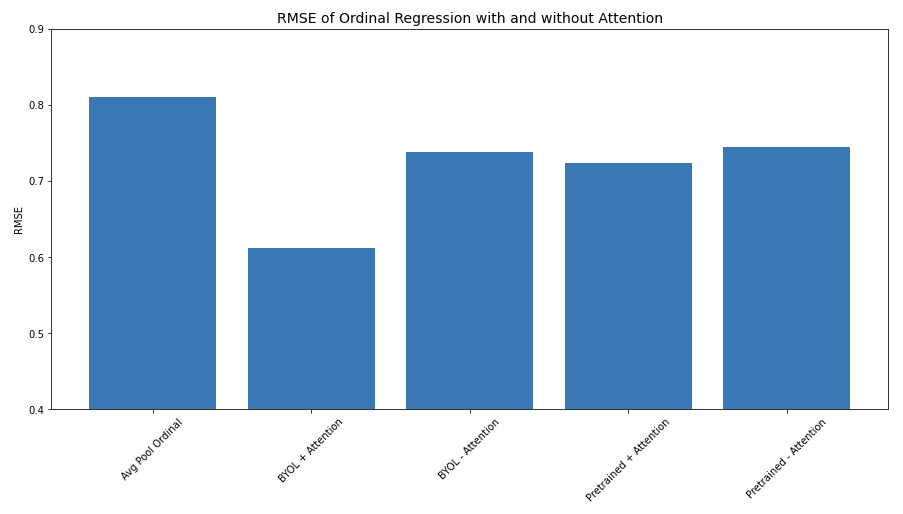
\includegraphics[scale=0.45]{acc_figure.png}
\end{center}
\caption{RMSE comparison of different model builds. (+ Attention) indicates the model includes attention pooling,
while (- Attention) means no attention pooling was used. Avg Pool Ordinal is a previous best, achieved using an ordinal Random Forest Regression on top of BYOL embeddings.}
\end{figure}

\subsection{Attention analysis}
In addition to evaluating our model through RMSE, we also investigated the points of high and low attention through the WSIs. To do so, we generated heatmaps of the WSIs, where each tile was replaced by its attention value. To do this we segmented a hold-out slide into tissue relevant tiles and passed each tile through the attention layer of our trained model and populated a map with the output attention value at its corresponding coordinates in the image. We found that the attention primarily focused on physiologically relevant areas to tau burden such as the Dentate Gyrus and CA1 (Figure 2). Interestingly, areas with dense white matter, such as the brain stem and neurofibril tracks, are given minimal attention. This is supportive of the underlying physiology of tau buildup and disease. 

\begin{figure}[h]
\begin{center}
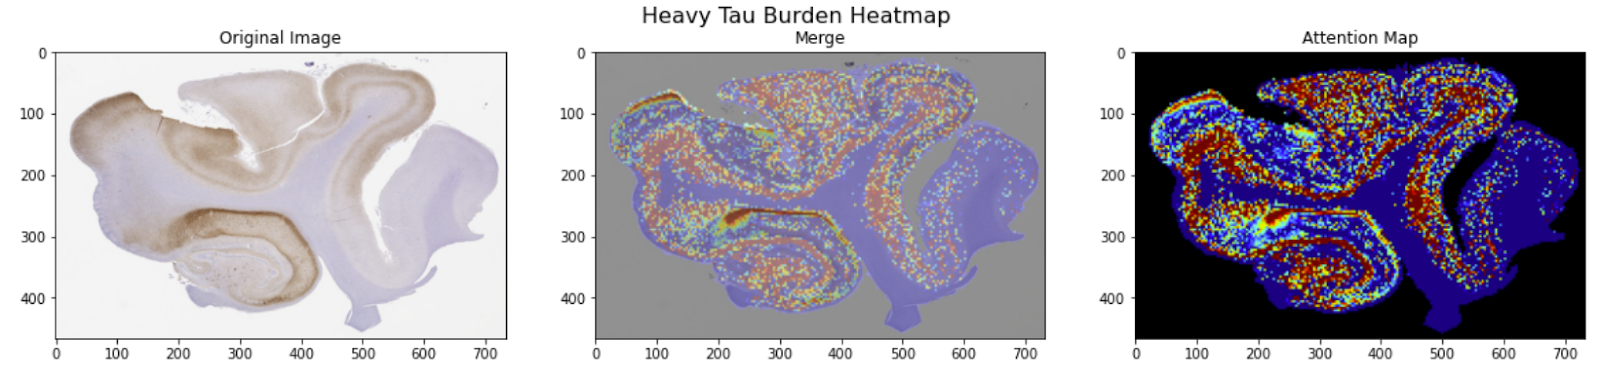
\includegraphics[scale=0.25]{attention_maps.png}
\end{center}
\caption{A representative attention heatmap of a Braak 3 image.}
\end{figure}

\section{Latent space analysis}
\label{lsa}

To investigate the quality of our feature space we employed k-means clustering and qualitatively assessed how well the clusters mapped onto the slide’s anatomy and pathology. We used this approach to directly compare the quality of feature vectors created by our BYOL model versus feature vectors created by the Resnet50 pretrained with Imagenet. Tile-level embeddings were first clustered using k-means. Then, each tile's cluster assignment was relayed back to its coordinates within the image, and plotted. The undoctored, original image is included in Figure 3.

\begin{figure}[h]
\begin{center}
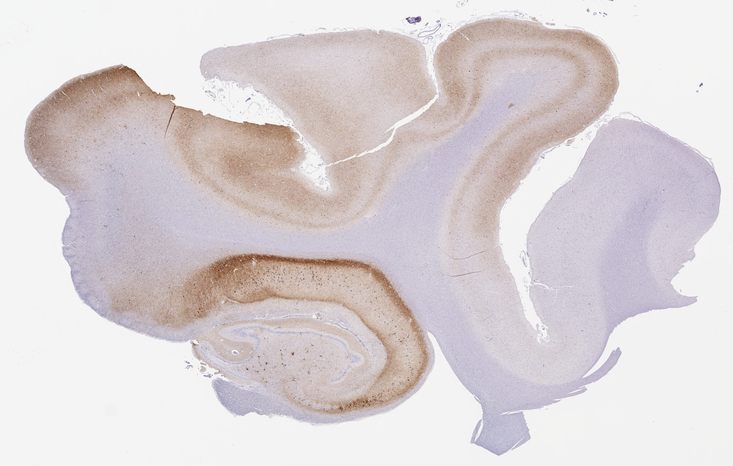
\includegraphics[scale=0.25]{wsi_undoctored.png}
\end{center}
\caption{A representative Braak 3 WSI.}
\end{figure}

\begin{figure}[h]
\begin{center}
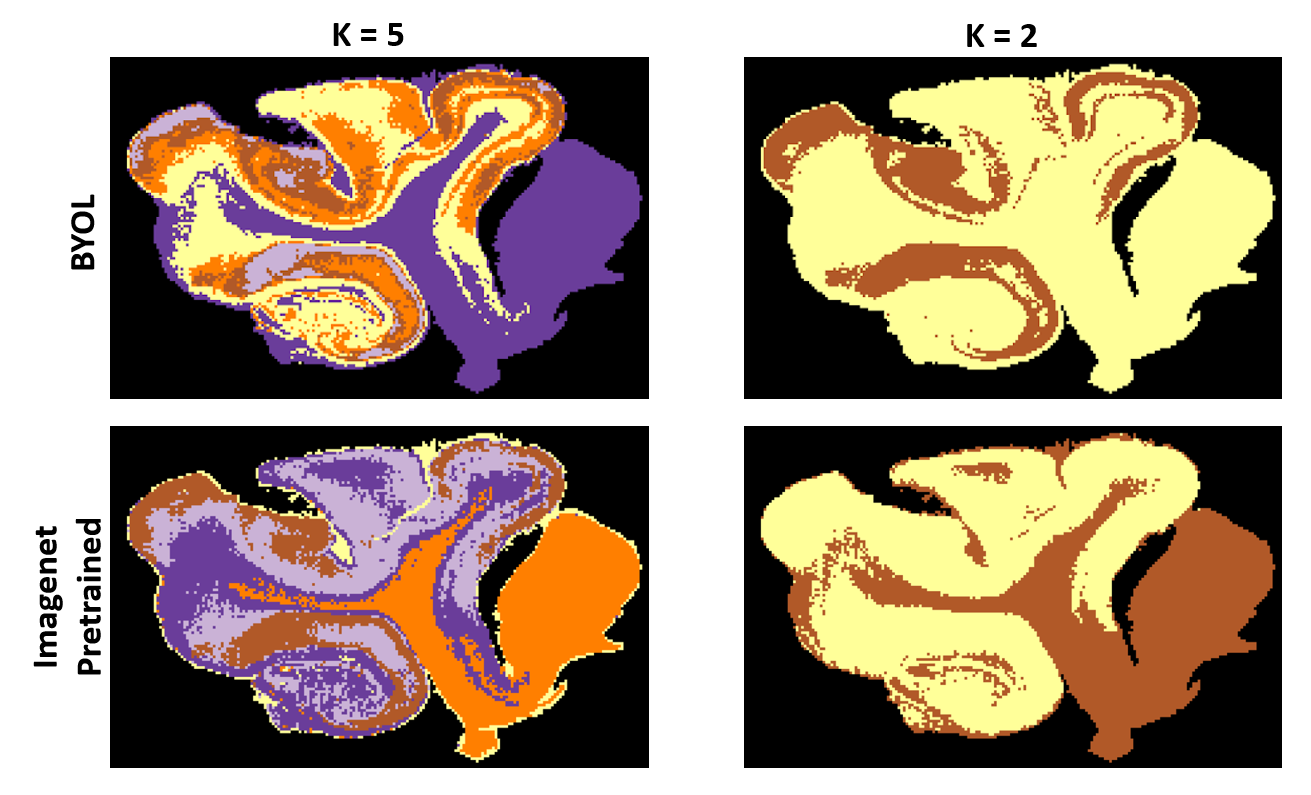
\includegraphics[scale=0.55]{cluster_comp.png}
\end{center}
\caption{Clustering Classifications of both BYOL and imagenet-pretrained embeddings. A \(k\) value of 2 and 5 were selected due to the major observable features in the image. \(K\) of 5 was selected in attempts to retrieve anatomical information, whereas \(k\) of 2 was selected to reveal tiles which possessed tangles.}
\end{figure}

As shown by the clustering maps (Figure 4), our BYOL embeddings encode much richer information than the imagenet pretrained embeddings. In \(k=2\) clusters, we can see that the tangle-laden tiles are much more accurately identified. Similarly, in \(k=5\) clusters, anatomical differences within the regions are much more distint within our BYOL embeddings. Interestingly, when paired with the attention heatmaps, cluster 3 (yellow) contains the most important areas for Braak classification. 

\section{Discussion}
Our implementation of trained attention as a means of transforming between tile-level space to slide-level space showed to greatly improve our model’s ability to predict a given hippocampal slide’s Braak score, as measured by a significant decrease in RMSE compared to our model which averaged tile feature vectors into a single slide-level feature vector . Furthermore, our generated attention heat maps show that the attention layer was properly using relevant pathology and anatomy, with the highest attention values being in areas densely packed with neurofibrillary tangles and the lowest attention values being in the white matter and vasculature which are least relevant to Braak scoring. 

Moving forward, we feel that our paradigm could be most greatly improved by implementing information regarding topography and anatomy into the model. One major issue with our current pooling methods is that they destroy all spatial information within the slides. Relative tangle location and other topographic information could prove crucial in a fully realized model of Braak scores. One solution to this is to log the location of each tile, and recreate the WSI as an “image of embeddings”, where each embedding is at the location of its respective tiles. A small CNN or other model could then be trained atop these embedded images. This would preserve the spatiality of tau presence, and perhaps provide a more accurate model of tau burden in the brain. 

Another approach could be to take advantage of the apparent anatomic and topographic based clustering of k-means and integrate the tile-level cluster assignments into the model. One way to do this would be to pass the k-centroids through an attention layer and weight the tiles according to the attention values of the cluster assignments. 


\subsubsection*{Acknowledgments}

We would like to thank John Crary for supplying the resources and data to conduct this project. Additional thanks goes to Jana Fehr and the rest of the DL2021 team for their support throughout this project and an excellent course.

\subsubsection*{References}

\small{
[1] Grill, J., Strub, F., Altch'e, F., Tallec, C., Richemond, P.H., Buchatskaya, E., Doersch, C., Pires, B.A., Guo, Z.D., Azar, M.G., Piot, B., Kavukcuoglu, K., Munos, R., \& Valko, M. (2020). Bootstrap Your Own Latent: A New Approach to Self-Supervised Learning. {\it ArXiv, abs/2006.07733}.

[2] Campanella, G., Hanna, M.G., Geneslaw, L. Miraflow, A., Krauss Silva, VW, Busam, KJ, Brogi, E., Reuter, VE, Klimstra, DS, \& Fuchs, TJ. (2019) Clinical-grade computational pathology using weakly supervised deep learning on whole slide images. {\it Nat Med} 25, 1301–130

[3] Cao, W., Mirjalili, V., \& Raschka, S. (2019). Rank-consistent ordinal regression for neural networks. arXiv preprint arXiv:1901.07884, 1(6), 13

[4] Lu, M., Williamson, D.F., Chen, T., Chen, R., Barbieri, M., \& Mahmood, F. (2021). Data Efficient and Weakly Supervised Computational Pathology on Whole Slide Images. {\it Nature biomedical engineering}.
}

\end{document}
